\section{Simulazione}
\begin{frame}{Simulazione}
	Introduciamo la definizione di densità di clienti ad ogni step al fine di avere una misura della gestione dell'affluenza di clienti nel negozio per le simulazioni.
	
	La \textbf{densità} di clienti per step corrisponde al numero di clienti medio per ogni cassa; la densità allo step $i$ è:
	\[\text{density}_i = \frac{\# \text{ customers in the supermarket}}{\# \text{ open cashdesks}}\]

\end{frame}

\begin{frame}{Validazione}
	Simulazione con gli stessi parametri del lavoro di Antczak e altri\footnote{\textit{Data-driven simulation modeling of the checkout process in supermarkets: Insights for decision support in retail operations}, Antczak, Tomasz and Weron, Rafał and Zabawa, Jacek, 2020}: 
	\begin{itemize}
		\item 20 casse standard con code parallele
		\item 6 casse self-service
		\item No jockeying
	\end{itemize}	
	4 simulazioni, una per ogni strategia di scelta della coda
\end{frame}

\begin{frame}{Validazione}
	\begin{figure}[H]
		\centering
		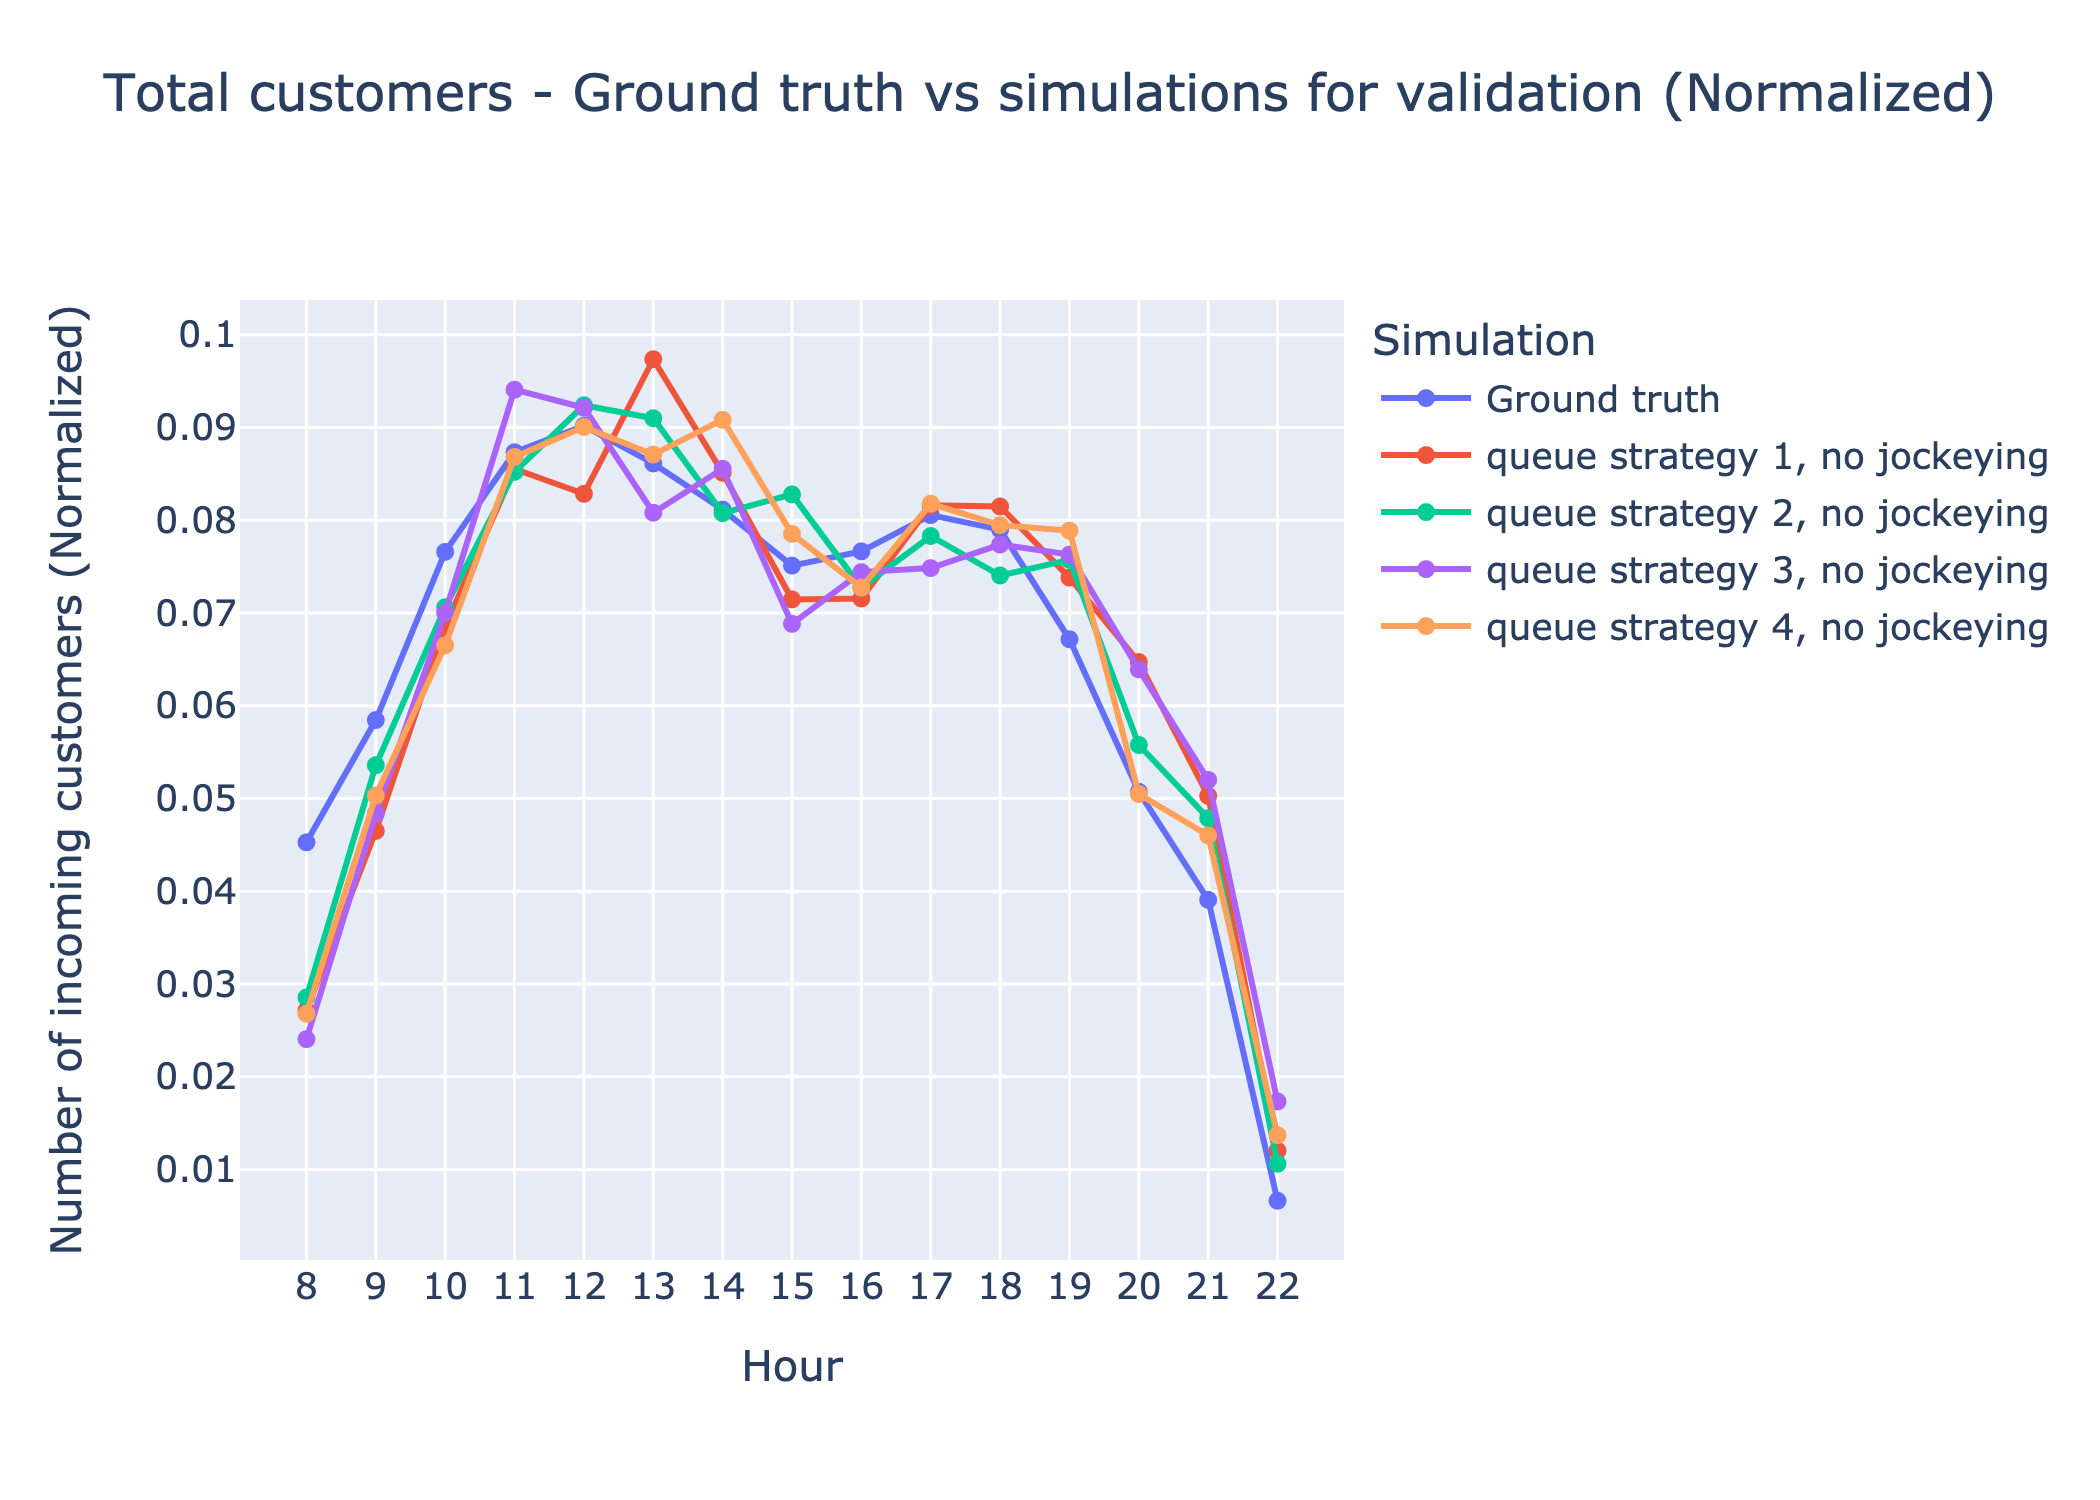
\includegraphics[width=8cm]{"../report/images/results/total_customers_validation.png"}
	\end{figure}
	A parità di parametri il nostro modello e quello dell'articolo sopportano allo stesso modo il numero di clienti nel negozio.
\end{frame}

\begin{frame}{Validazione}
	\begin{figure}[H]
		\centering
		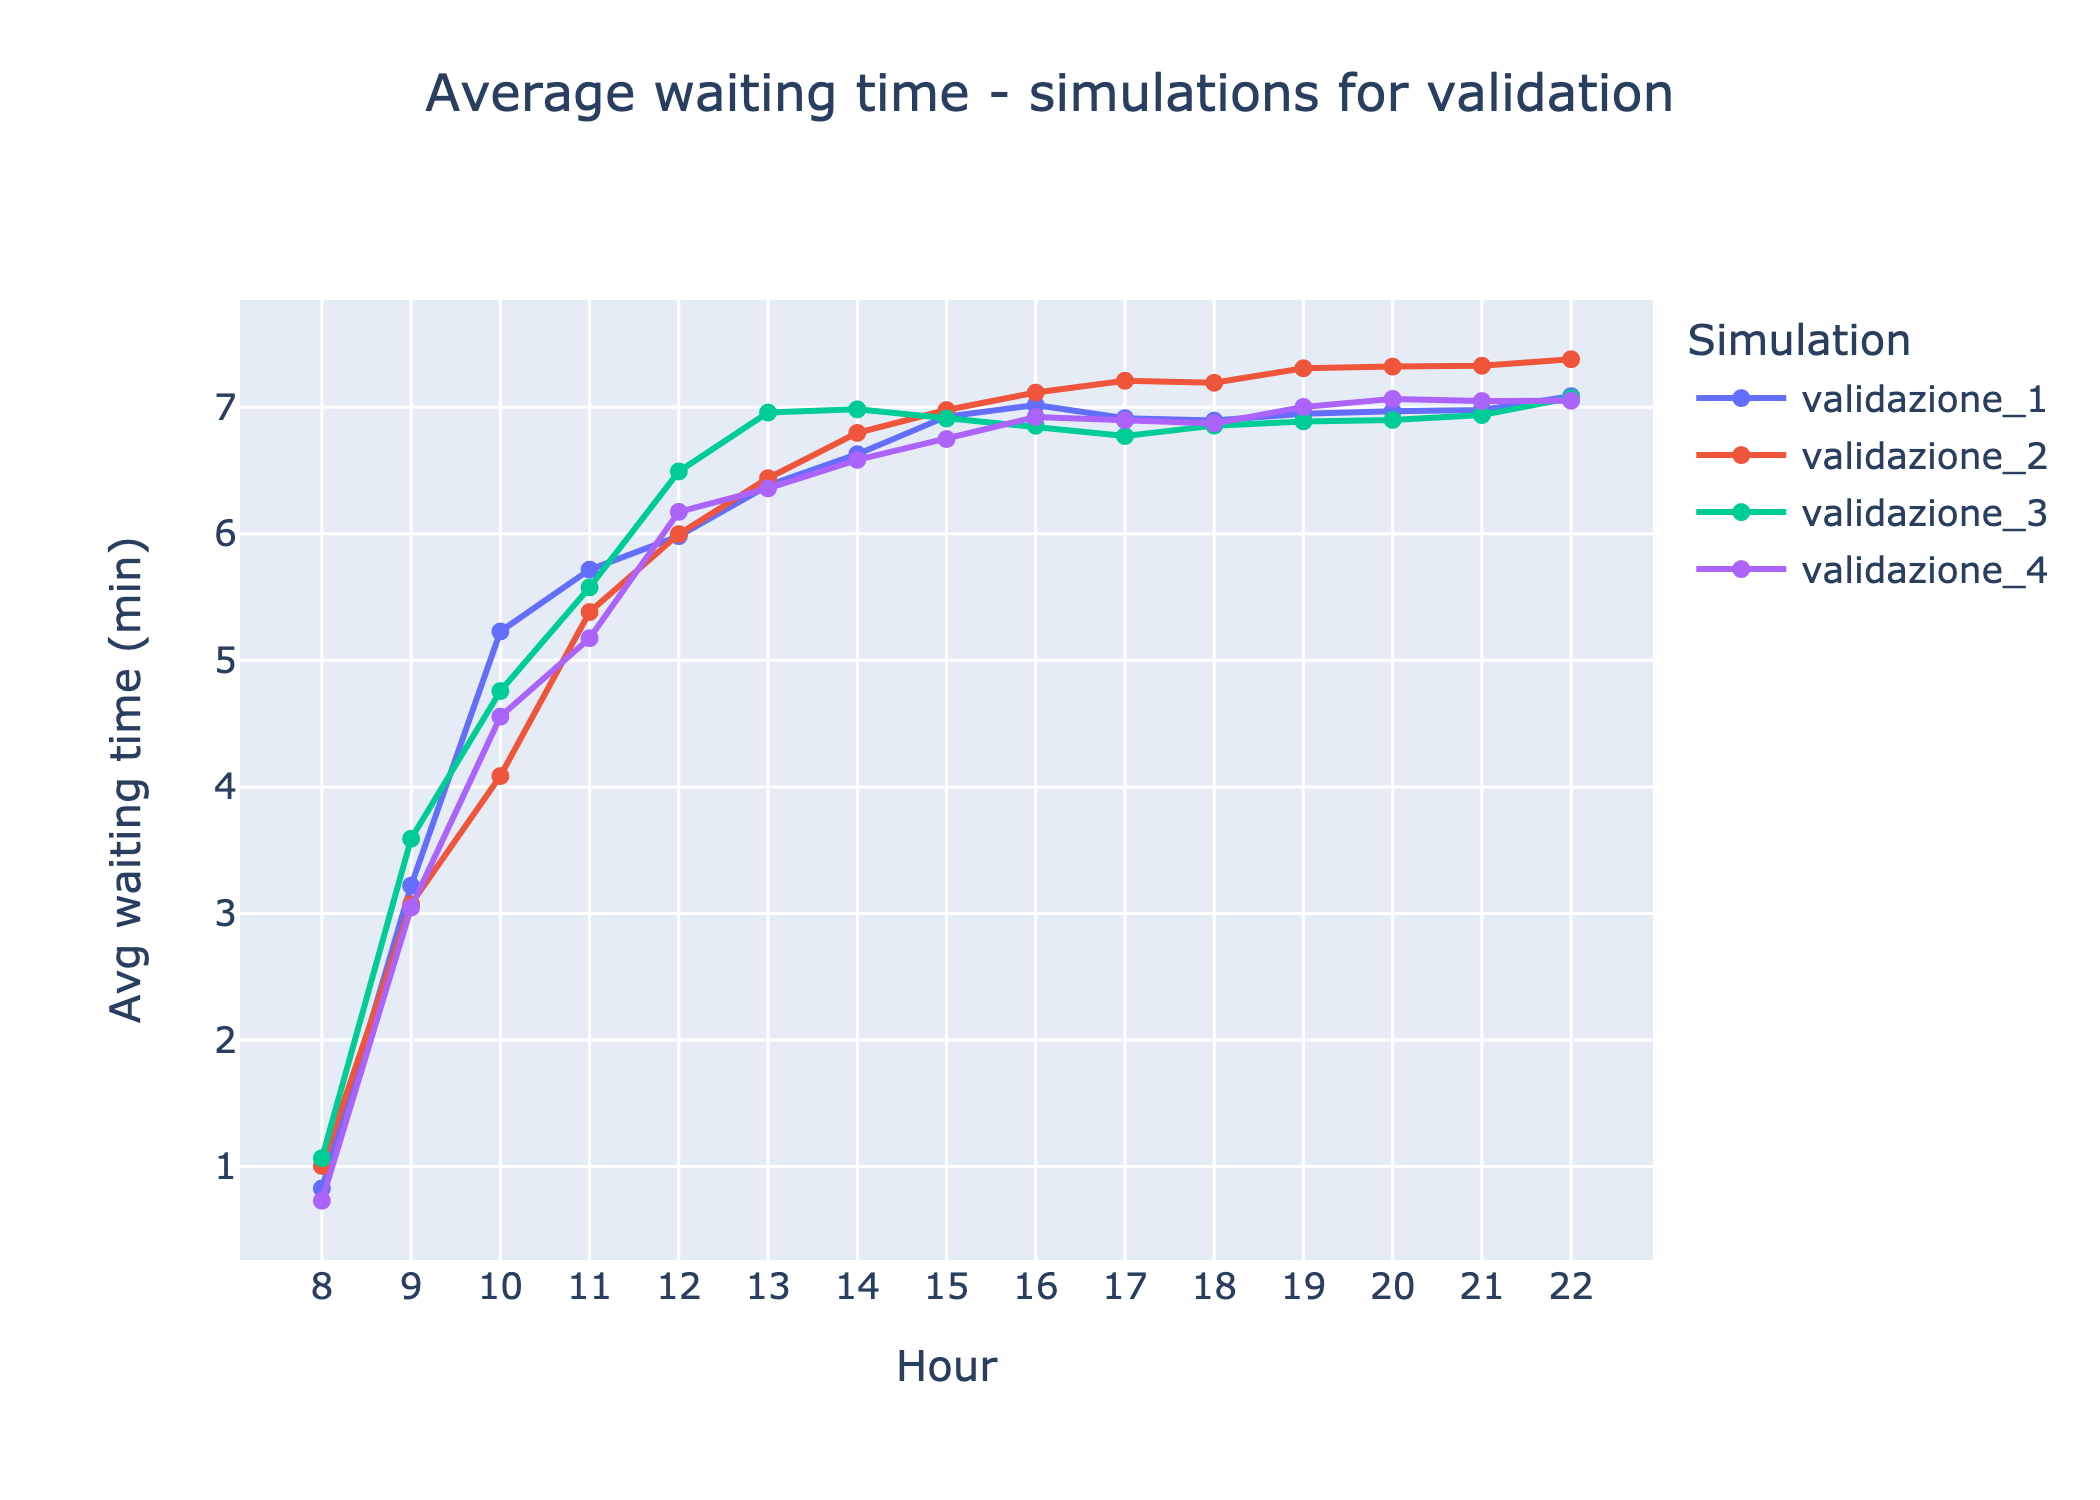
\includegraphics[width=8cm]{"../report/images/results/avg_wt_validation.png"}
	\end{figure}
	In assenza di jockey le strategie 3 e 4 sono quelle che tengono il tempo d'attesa medio più basso.
\end{frame}

\begin{frame}{Simulazione con jockey}
	Aggiungiamo le 2 strategie di jockey. I parametri saranno quindi:
	\begin{itemize}
		\item 20 casse normali con code parallele
		\item 6 casse self-service
		\item 4 strategie di scelta della coda
		\item 2 strategie di jockey
	\end{itemize}
	Per un totale di 8 simulazioni.
\end{frame}

\begin{frame}{Simulazione con jockey}
	\begin{figure}[H]
		\centering
		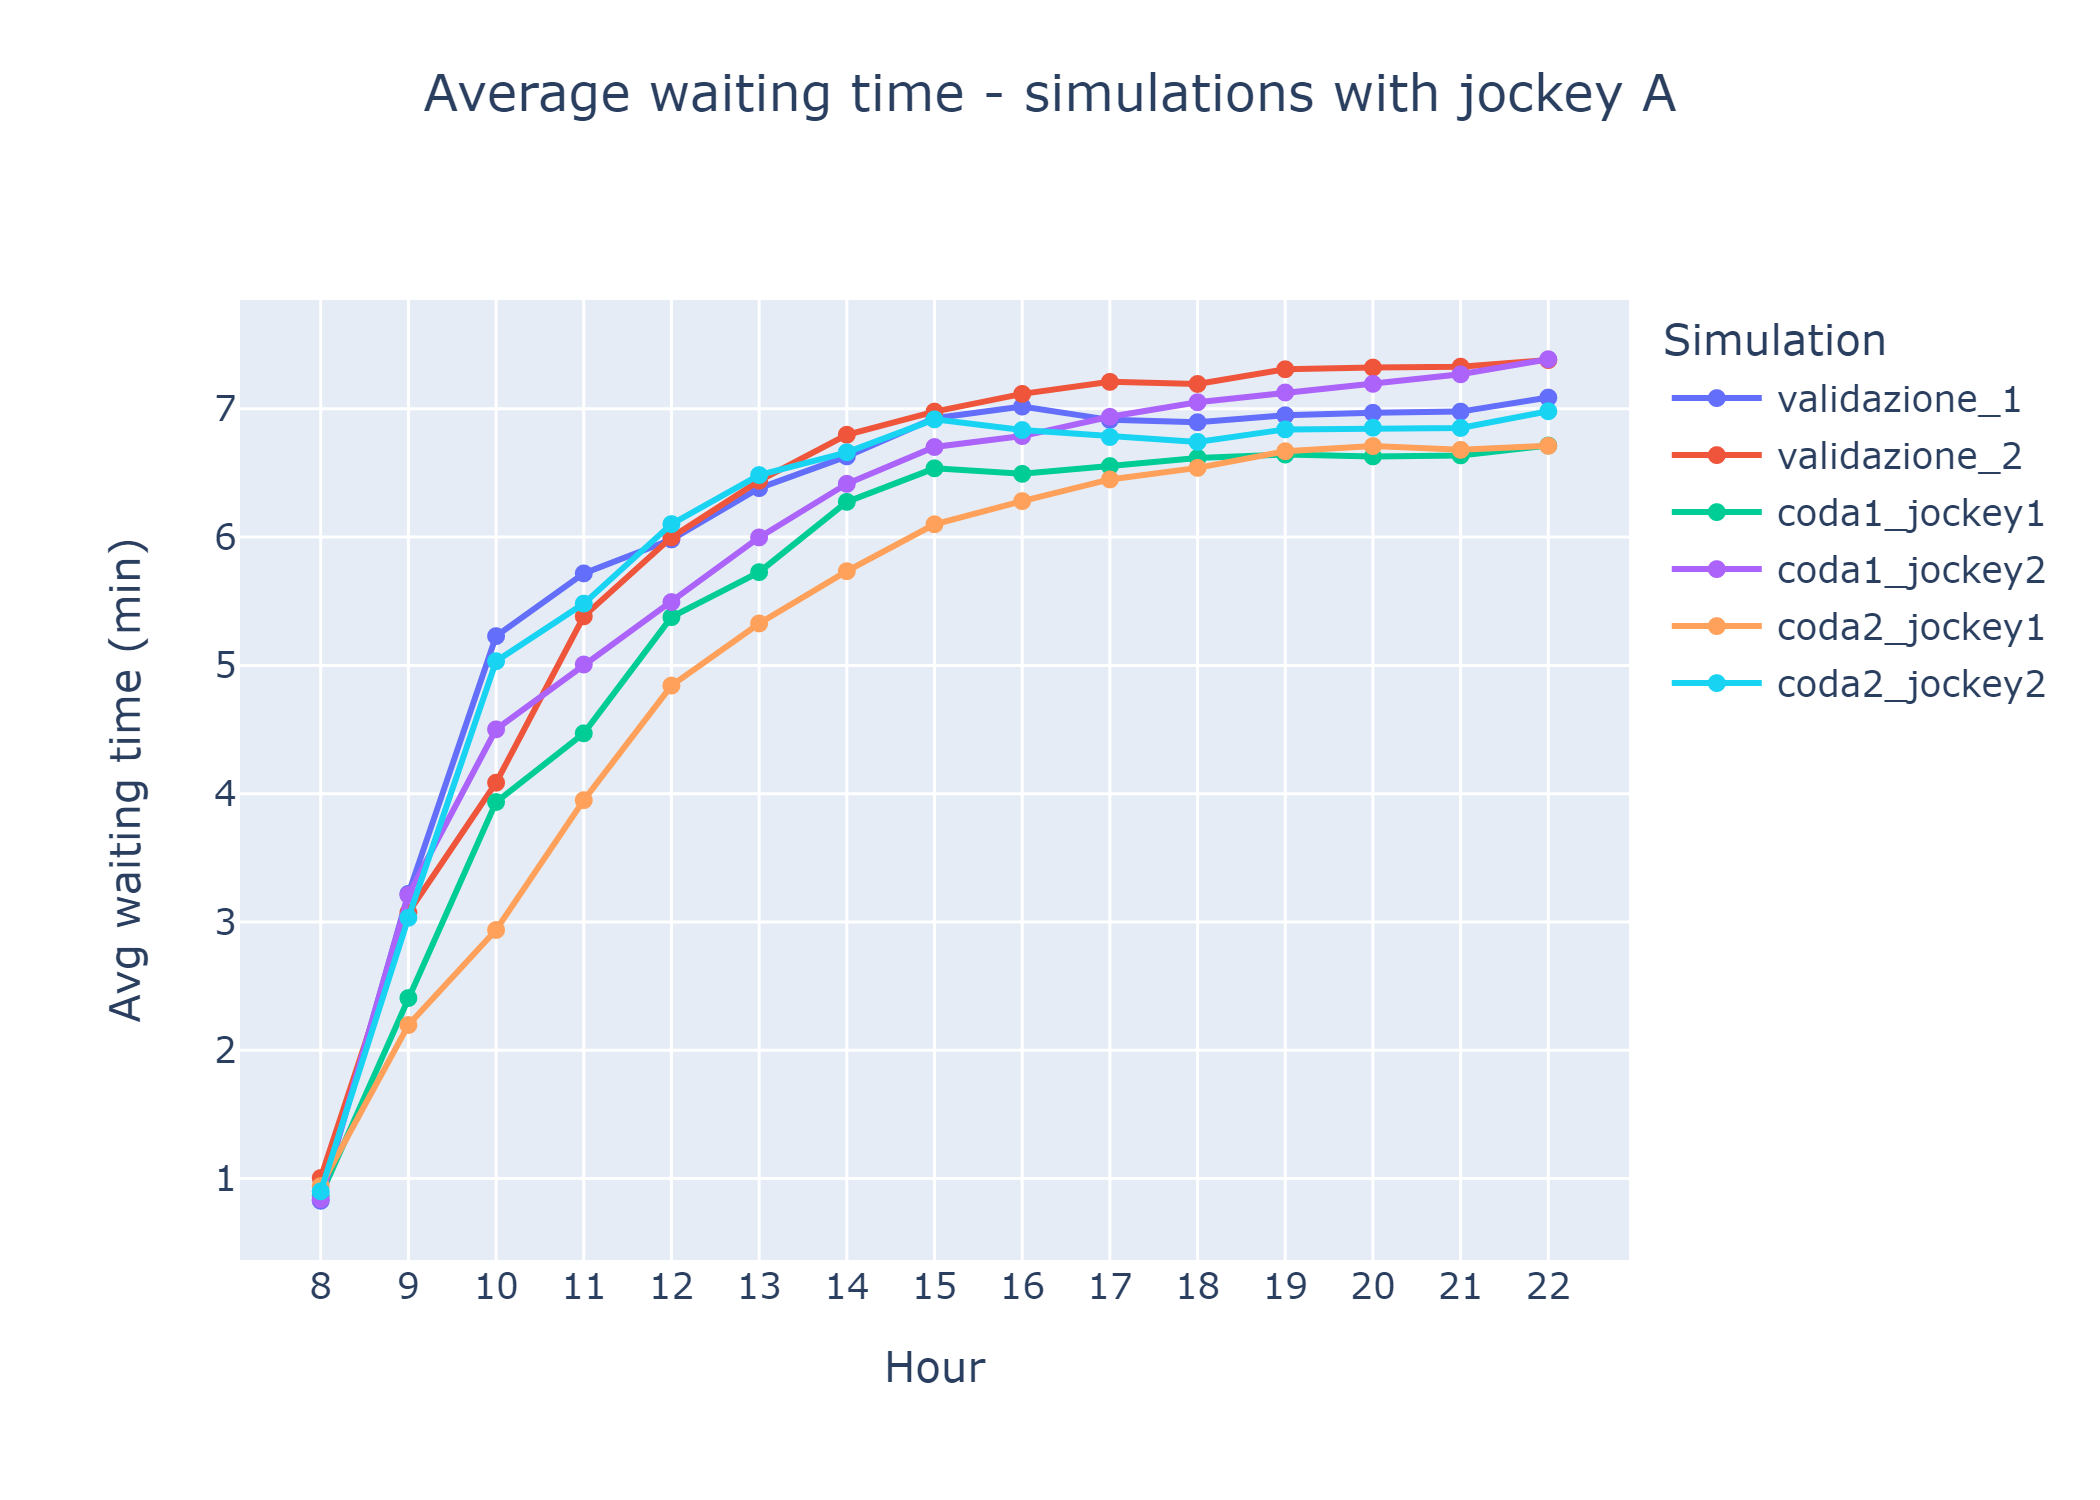
\includegraphics[width=8cm]{"../report/images/results/avg_wt_jockey_a.png"}
	\end{figure}
	I risultati migliori si raggiungono quando la strategia di scelta della coda e di jockey sono la stessa. In ogni caso fare jockey è sempre conveniente.
\end{frame}

\begin{frame}{Simulazione con jockey}
	\begin{figure}[H]
		\centering
		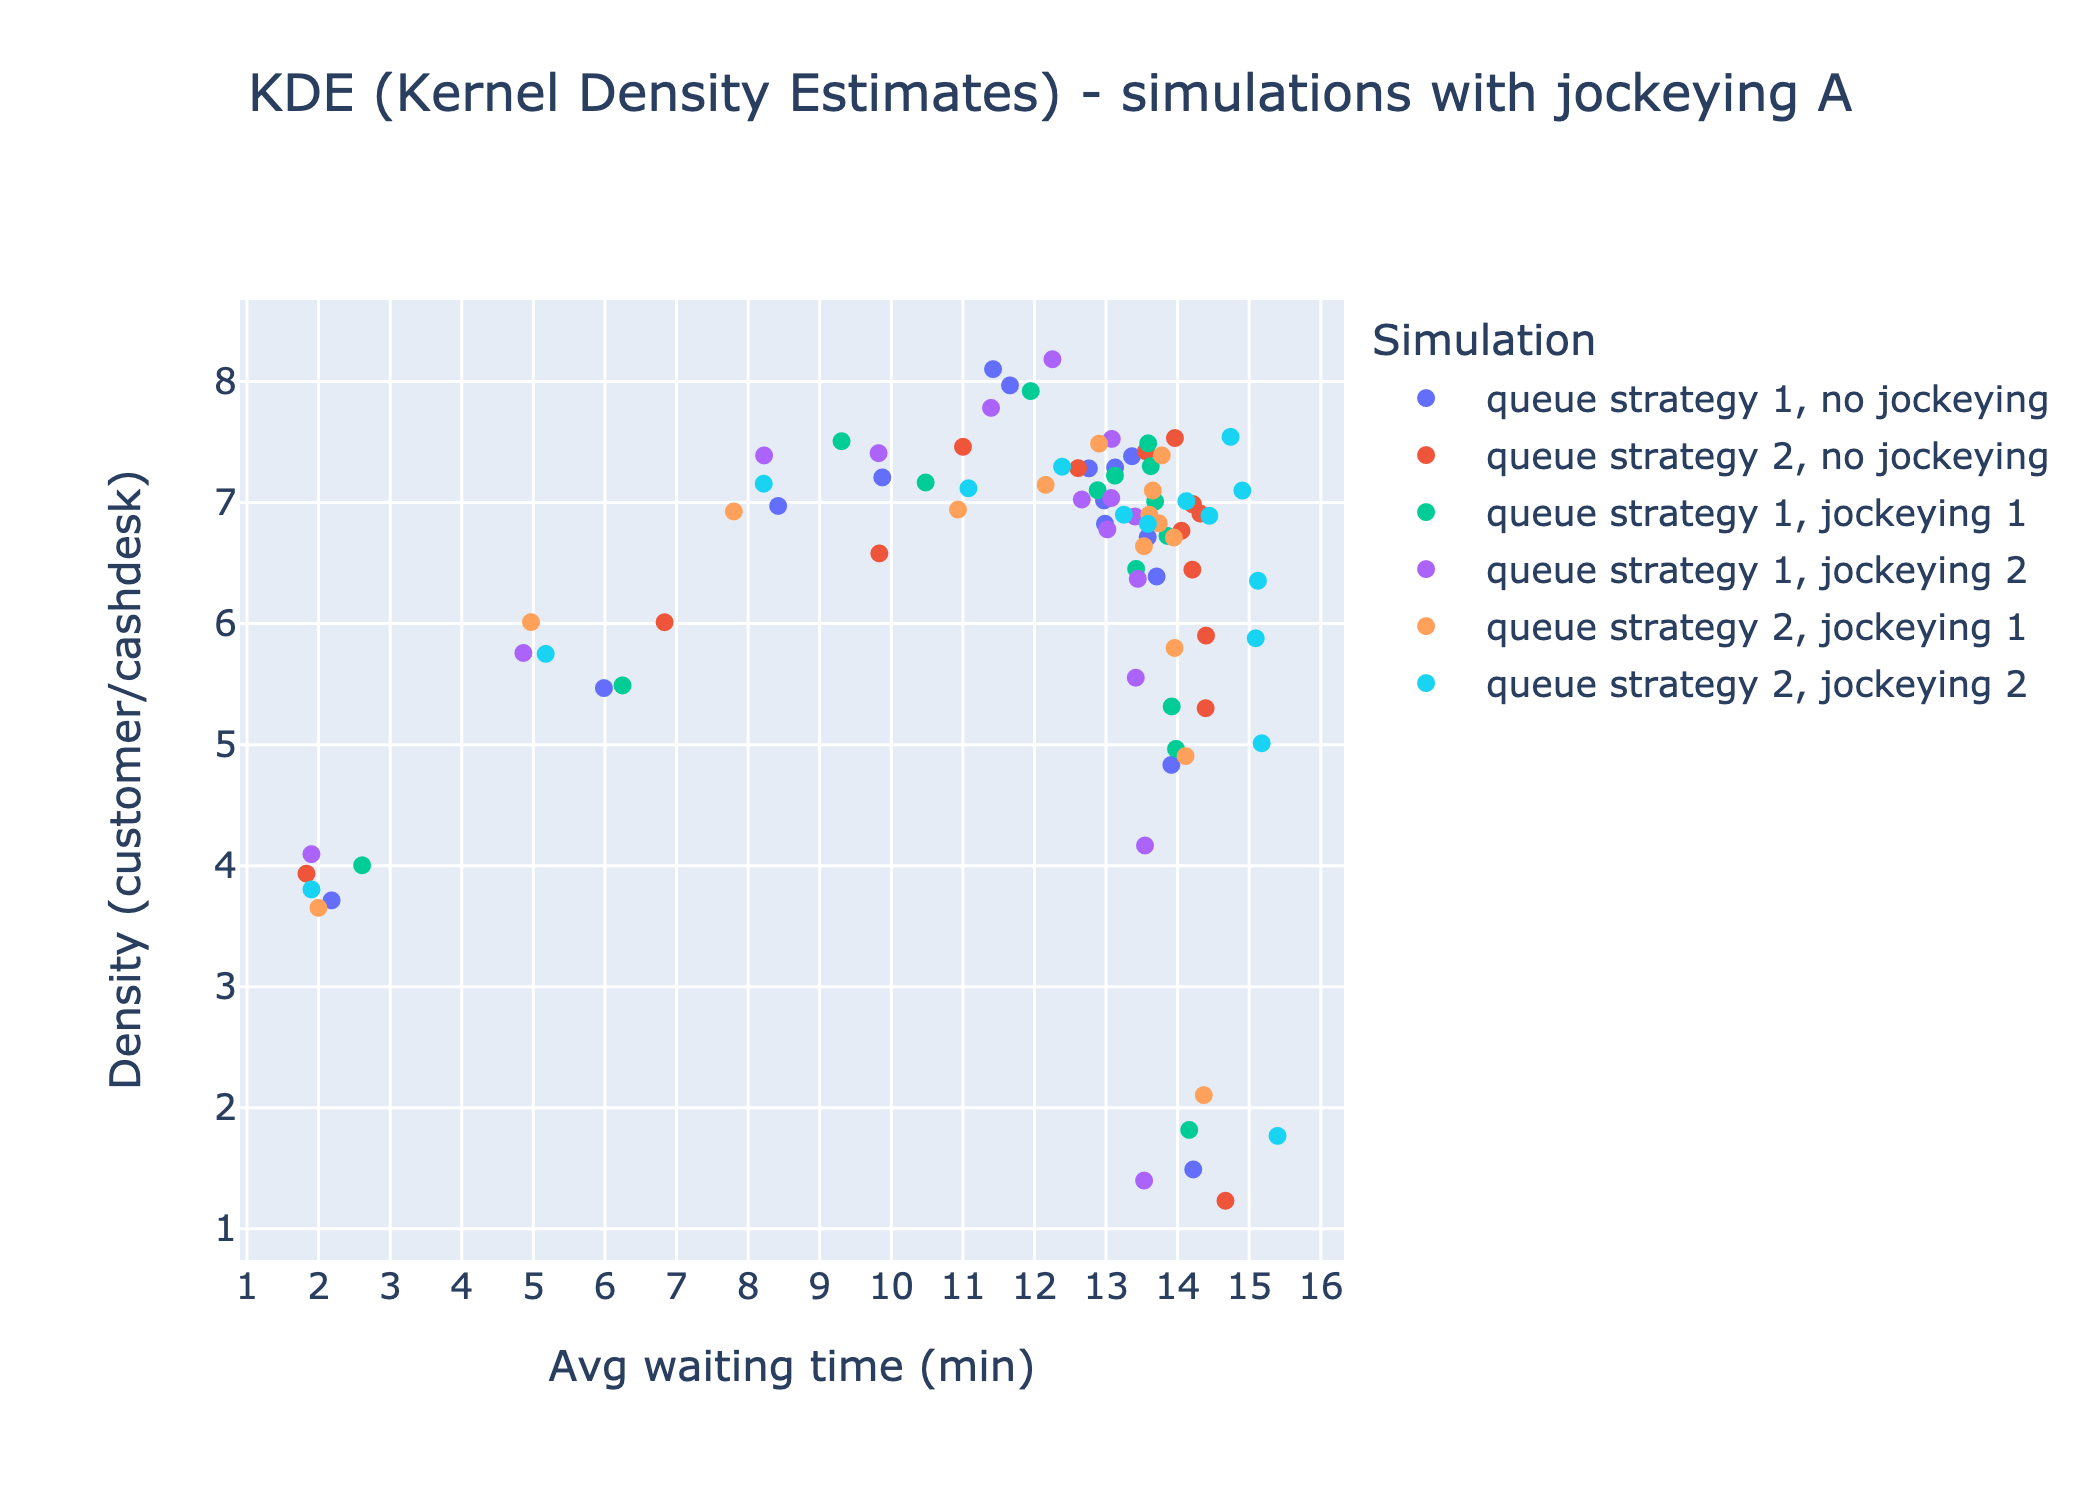
\includegraphics[width=8cm]{"../report/images/results/kde_jockey_a.png"}
	\end{figure}
	Si raggiunge un punto critico di densità dopo il quale il sistema reagisce e permette alle code di scorrere abbassando il tempo d'attesa.
\end{frame}

\begin{frame}{Simulazione con jockey}
	\begin{figure}[H]
		\centering
		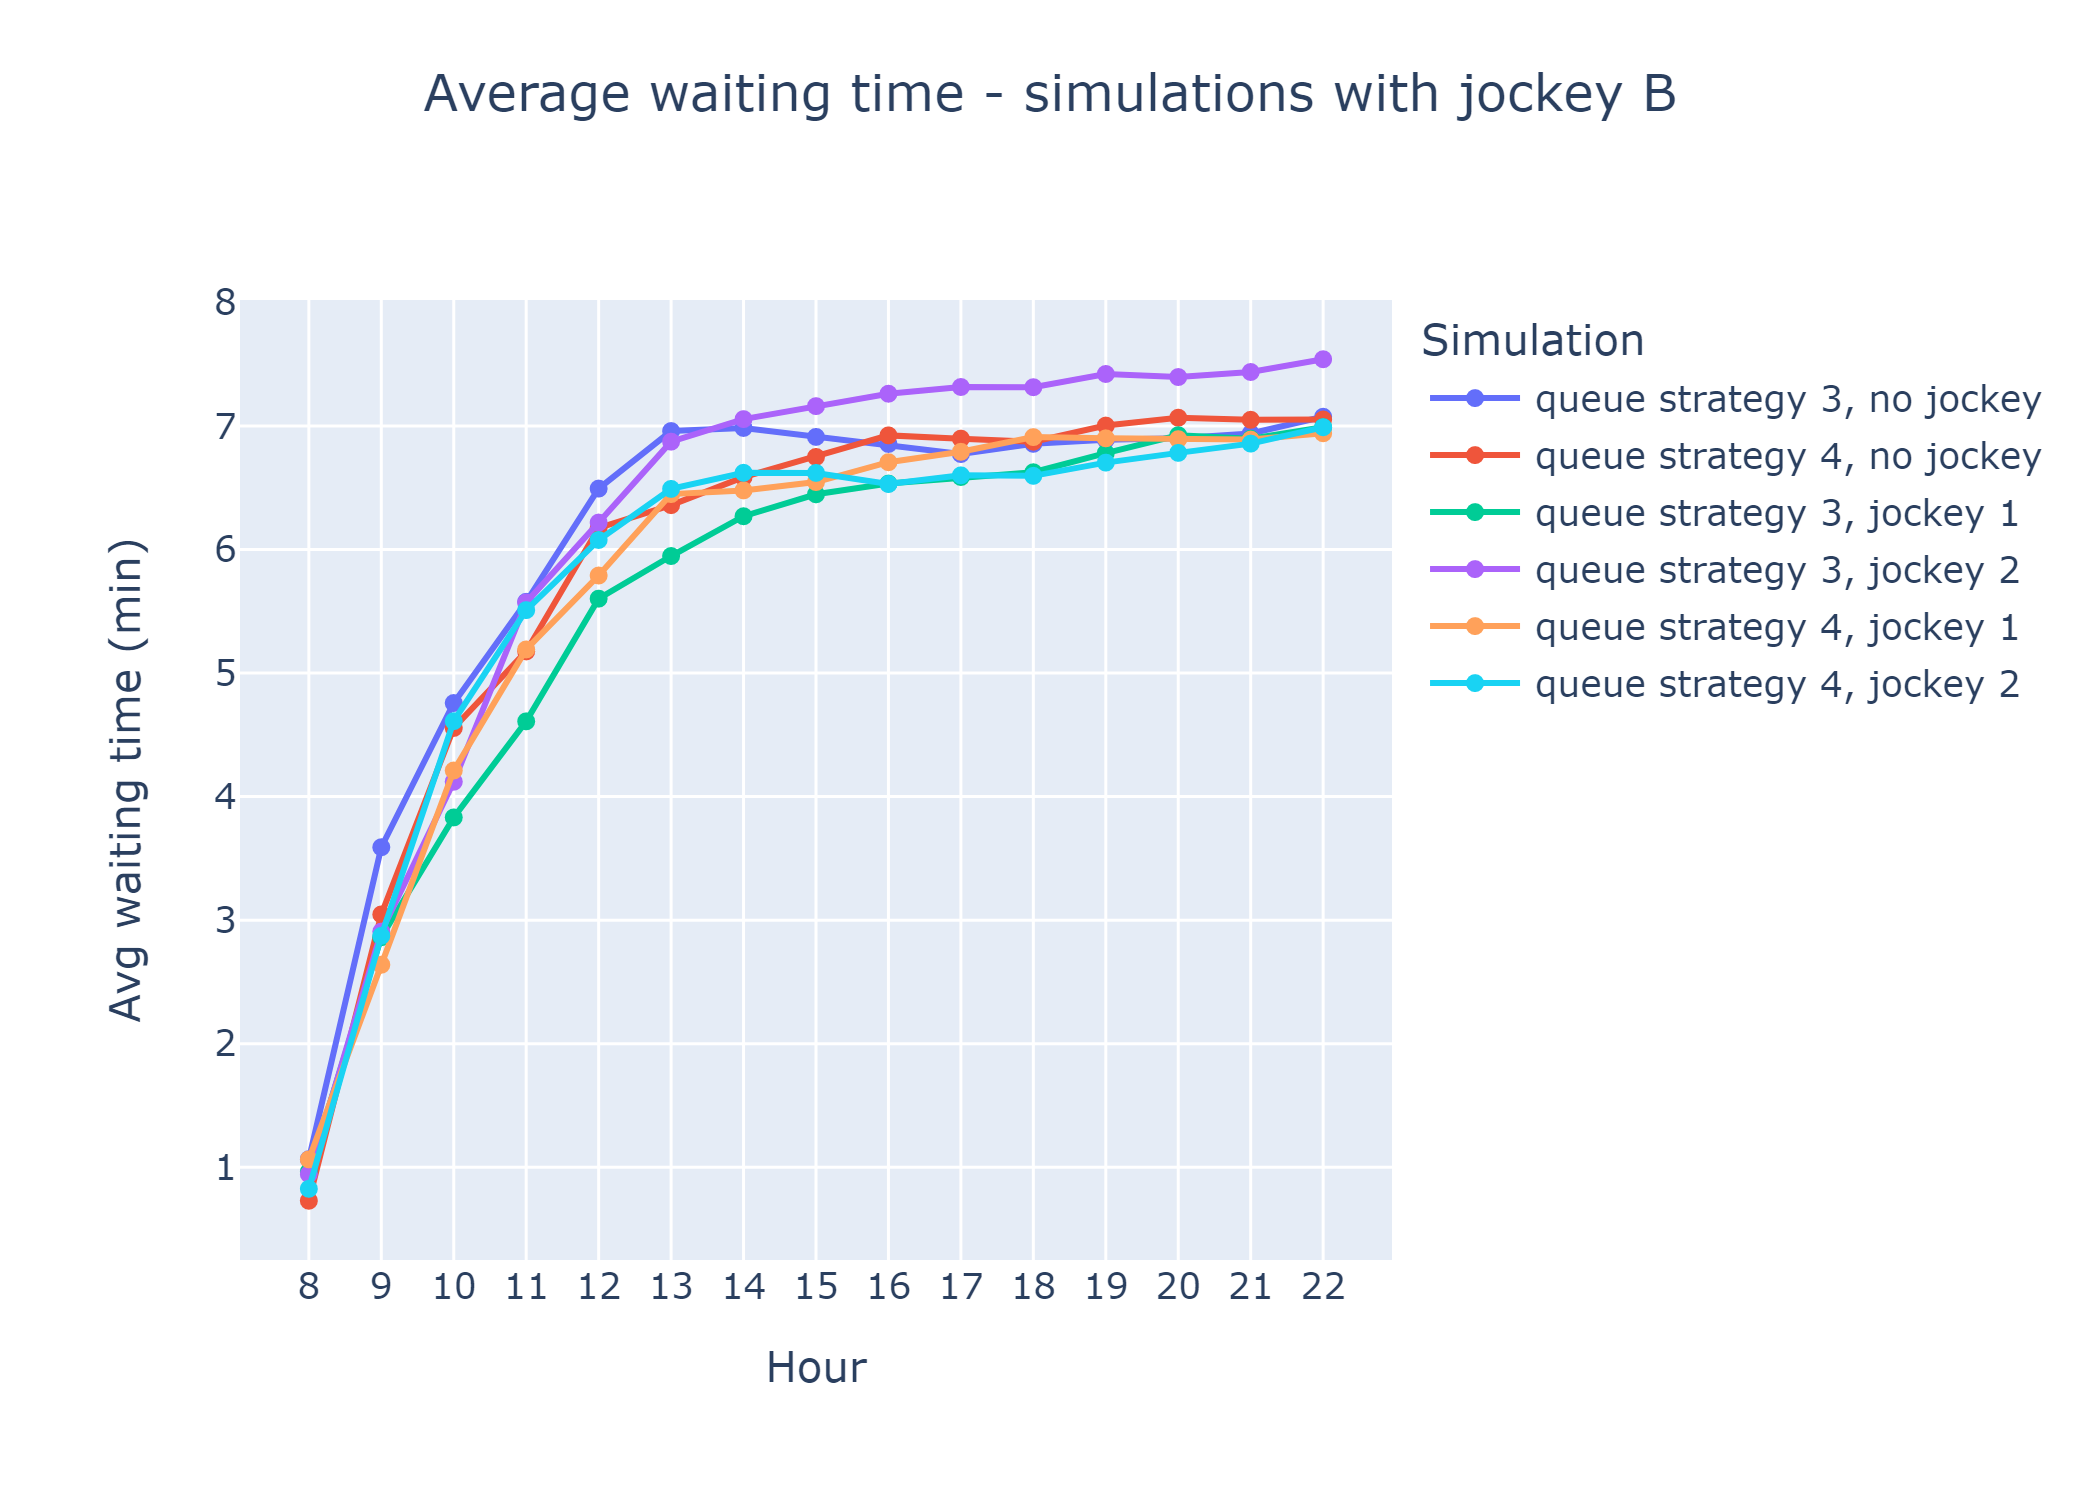
\includegraphics[width=8cm]{"../report/images/results/avg_wt_jockey_b.png"}
	\end{figure}
	La migliore è la strategia di scelta della coda in base alla power regression con jockey in base al numero di elementi. Non si può dire quanto detto sopra perchè la strategia di jockey non è la stessa.
\end{frame}

\begin{frame}{Simulazione con jockey}
	\begin{figure}[H]
		\centering
		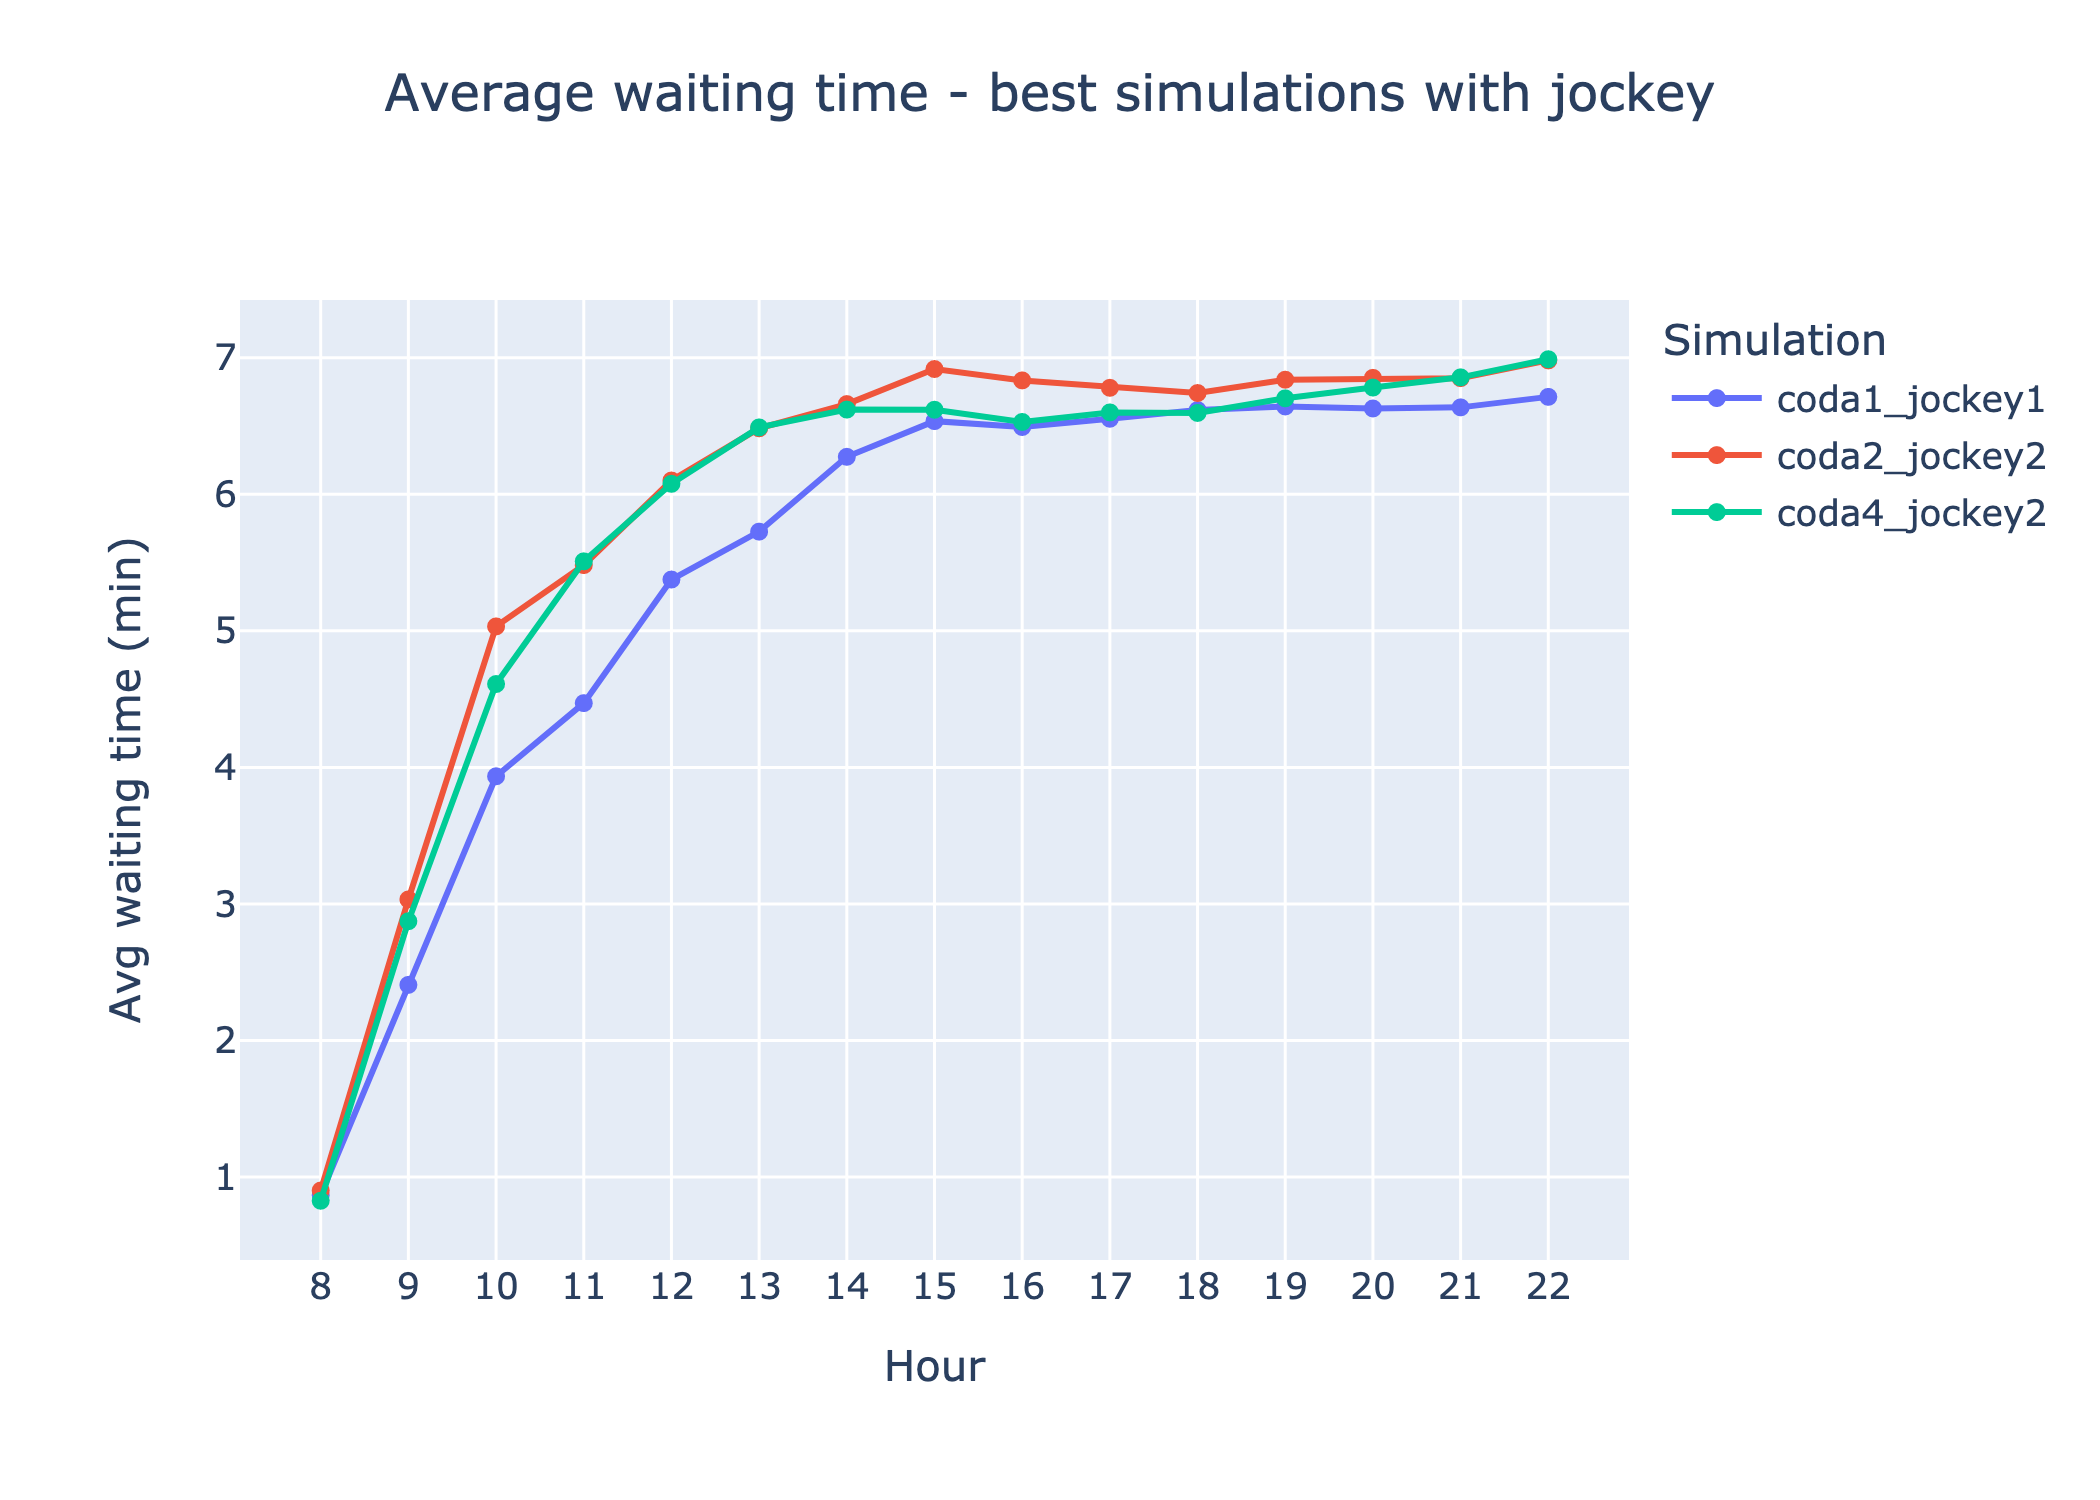
\includegraphics[width=8cm]{"../report/images/results/avg_wt_jockey_best.png"}
	\end{figure}
	Le migliori 3 strategie di scelta della coda fino ad ora. La prima strategia rimane sempre quella con il tempo medio d'attesa minore.
\end{frame}

\begin{frame}{Simulazione con coda condivisa}
	Mettiamo a confronto le code parallele con l'N-fork.\\
	Osservando le simulazioni già fatte ci accorgiamo che il numero massimo di casse aperto in un istante è 8, per questo indaghiamo i casi con 5, 6, 7 e 8 casse.
\end{frame}

\begin{frame}{Simulazione con coda condivisa}
	\begin{figure}[H]
		\centering
		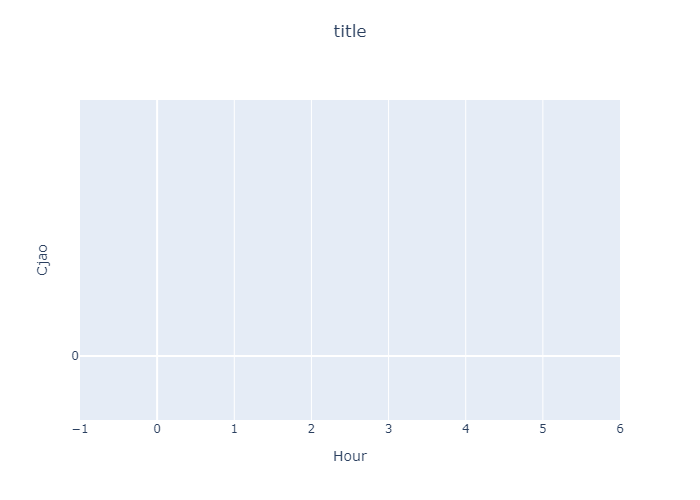
\includegraphics[width=8cm]{"../report/images/results/avg_wt_codacondivisa.png"}
	\end{figure}
	5 casse sono troppo poche sia per le code parallele che per l'N-fork. Si nota la divisione netta tra i tempi d'attesa delle due configurazioni nel caso di 6, 7 e 8 casse.
\end{frame}

\begin{frame}{Simulazione con coda condivisa}
	\begin{figure}[H]
		\centering
		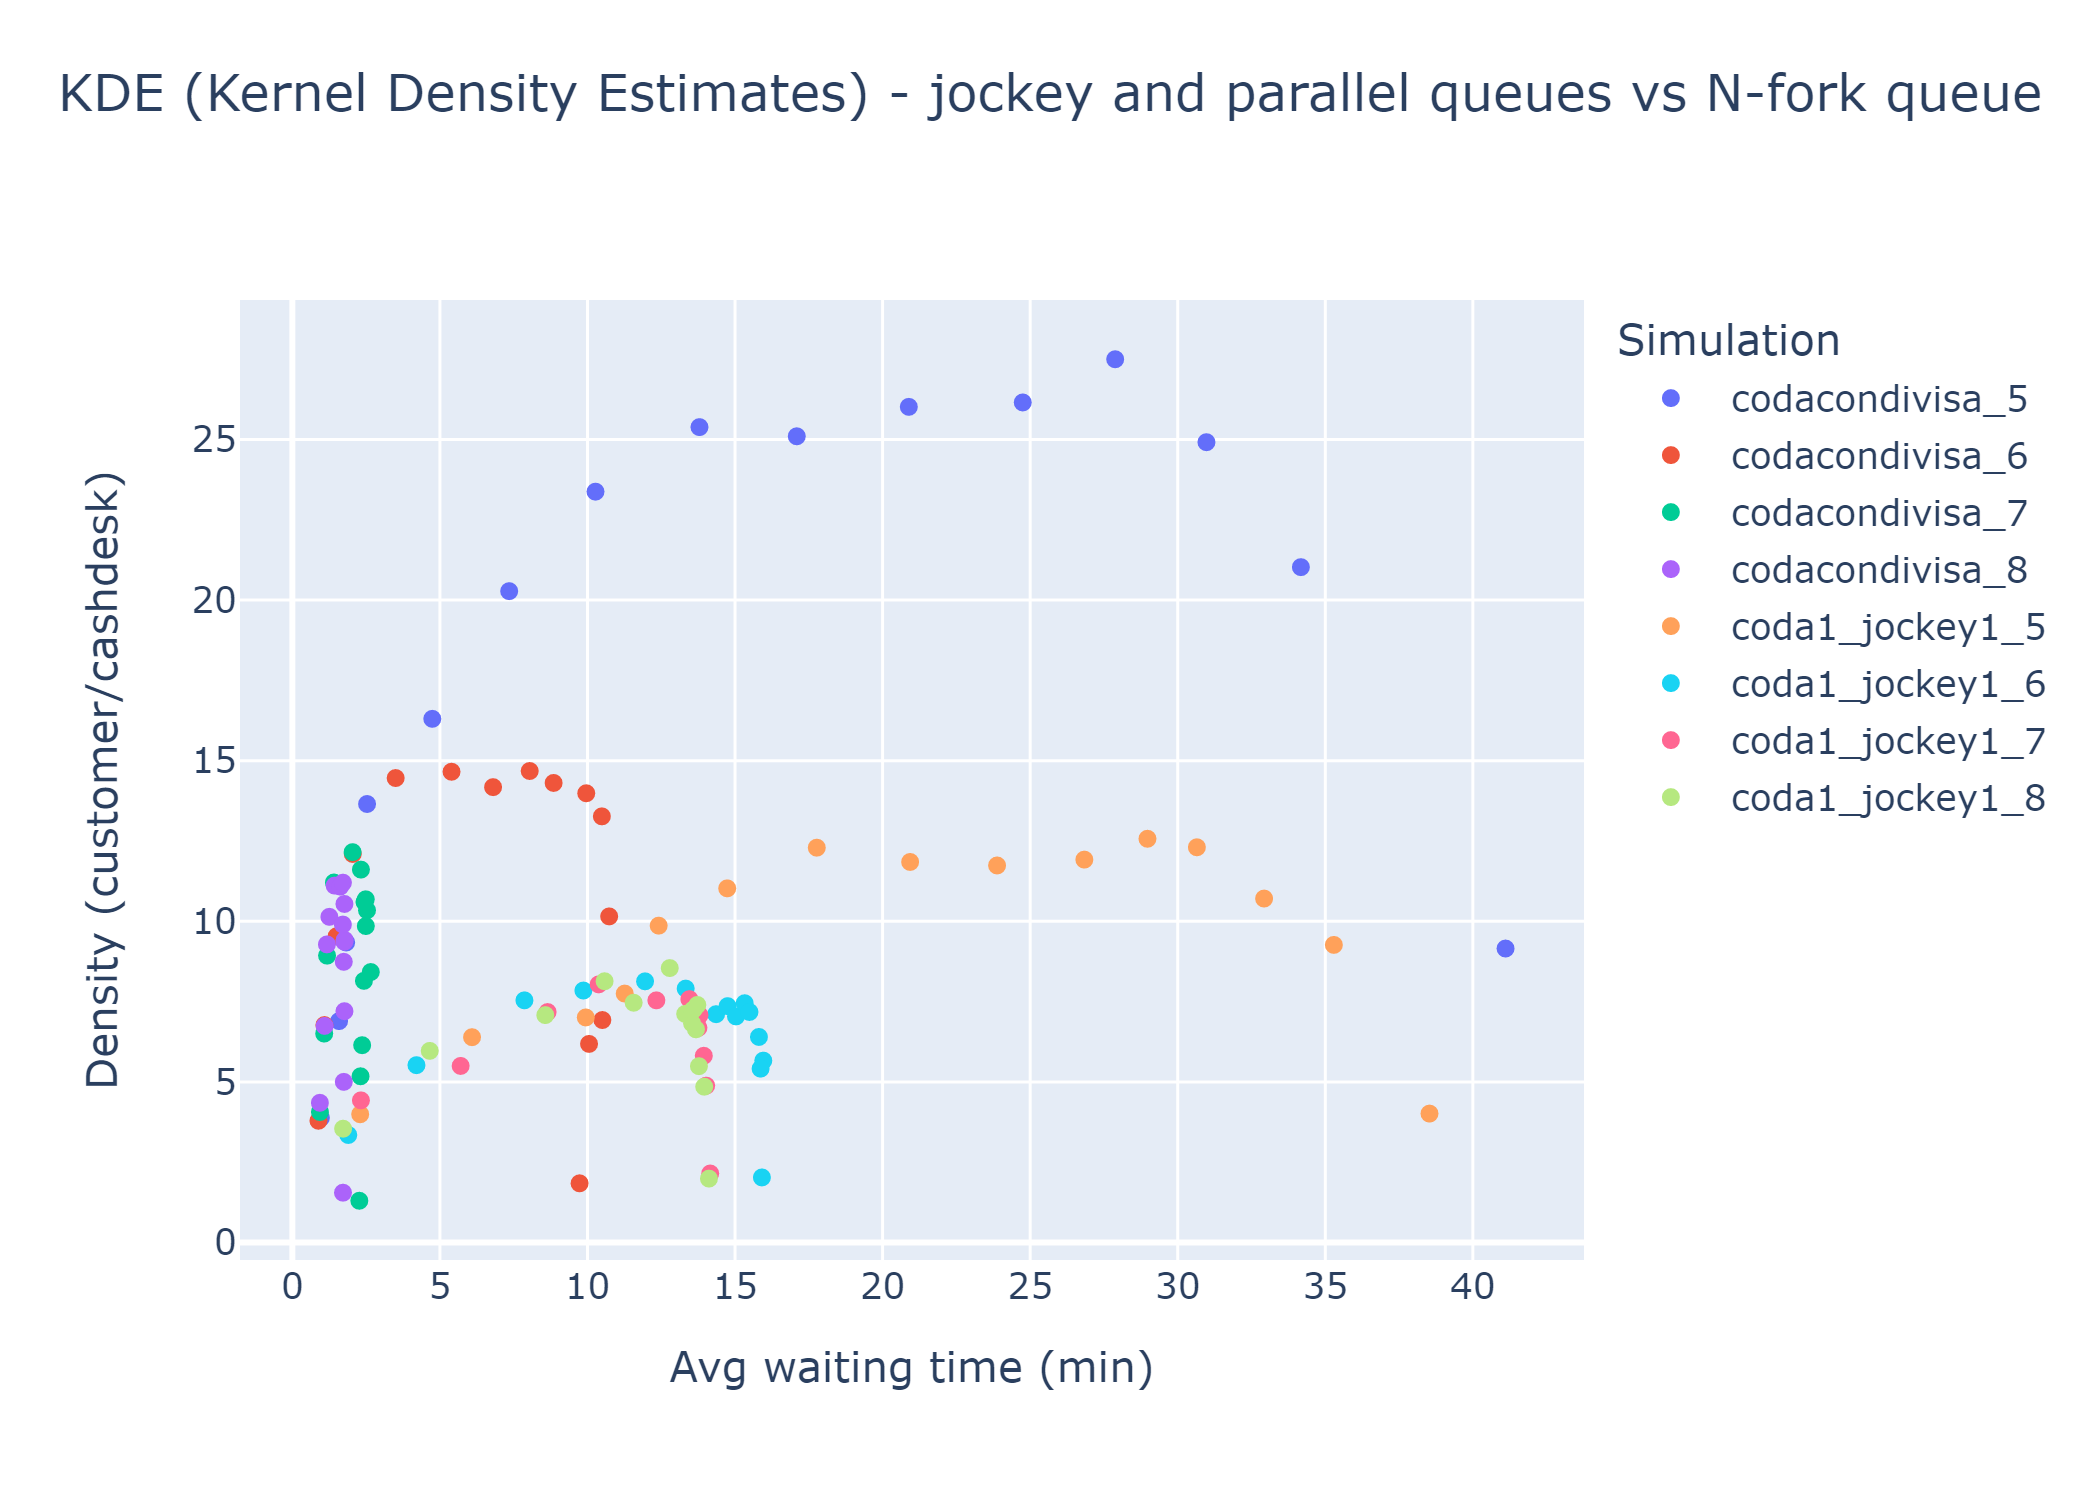
\includegraphics[width=8cm]{"../report/images/results/kde_codacondivisa.png"}
	\end{figure}
	Di nuovo 5 casse sono troppo poche. La coda condivisa arriva a densità molto più alte, questo è un limite del modello, infatti quando la fila si riempie i clienti non possono mettersi in coda. In tutti i casi la coda condivisa sopporta più densità e abbassa i tempi medi.
\end{frame}

\begin{frame}{Simulazione con coda condivisa}
	\begin{figure}[H]
		\centering
		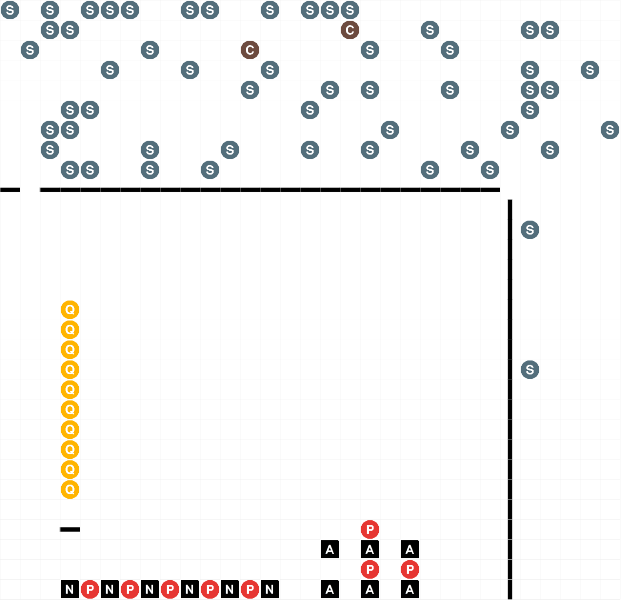
\includegraphics[width=5cm]{"../report/images/results/codacondivisa_screenshot.png"}
	\end{figure}
	Questo è un esempio di coda piena con clienti in attesa.
\end{frame}

\begin{frame}{Simulazione con casse self-scan}
	Simulazione con sole casse self-scan, in particolare 7. \\
	Le probabilità di rilettura sono:
	\begin{itemize}
		\item $97 \%$ nessuna rilettura
		\item $2 \%$ rilettura parziale
		\item $1 \%$ rilettura totale
	\end{itemize}
\end{frame}

\begin{frame}{Simulazione con casse self-scan}
	\begin{figure}[H]
		\centering
		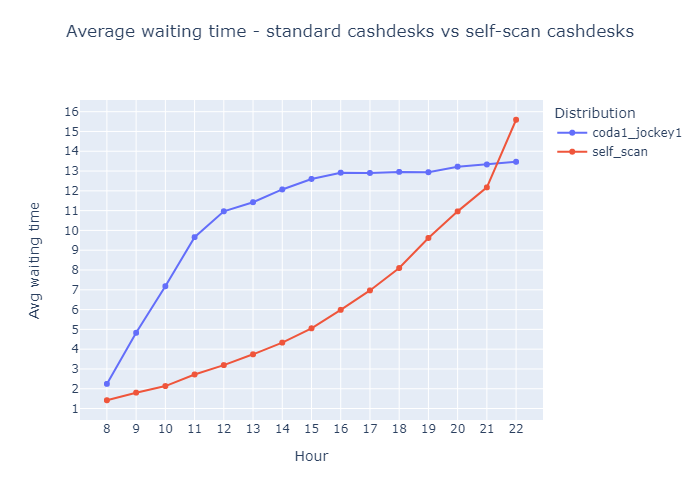
\includegraphics[width=8cm]{"../report/images/results/avg_wt_selfscan.png"}
	\end{figure}
	Il tempo d'attesa medio delle self-scan aumenta in modo esponenziale: la cassa riservata per le riletture è un collo di bottiglia. Bisognerebbe avere dei dati più completi sulla distribuzione di clienti self-scan.
\end{frame}

\begin{frame}{Simulazione con casse self-scan}
	\begin{figure}[H]
		\centering
		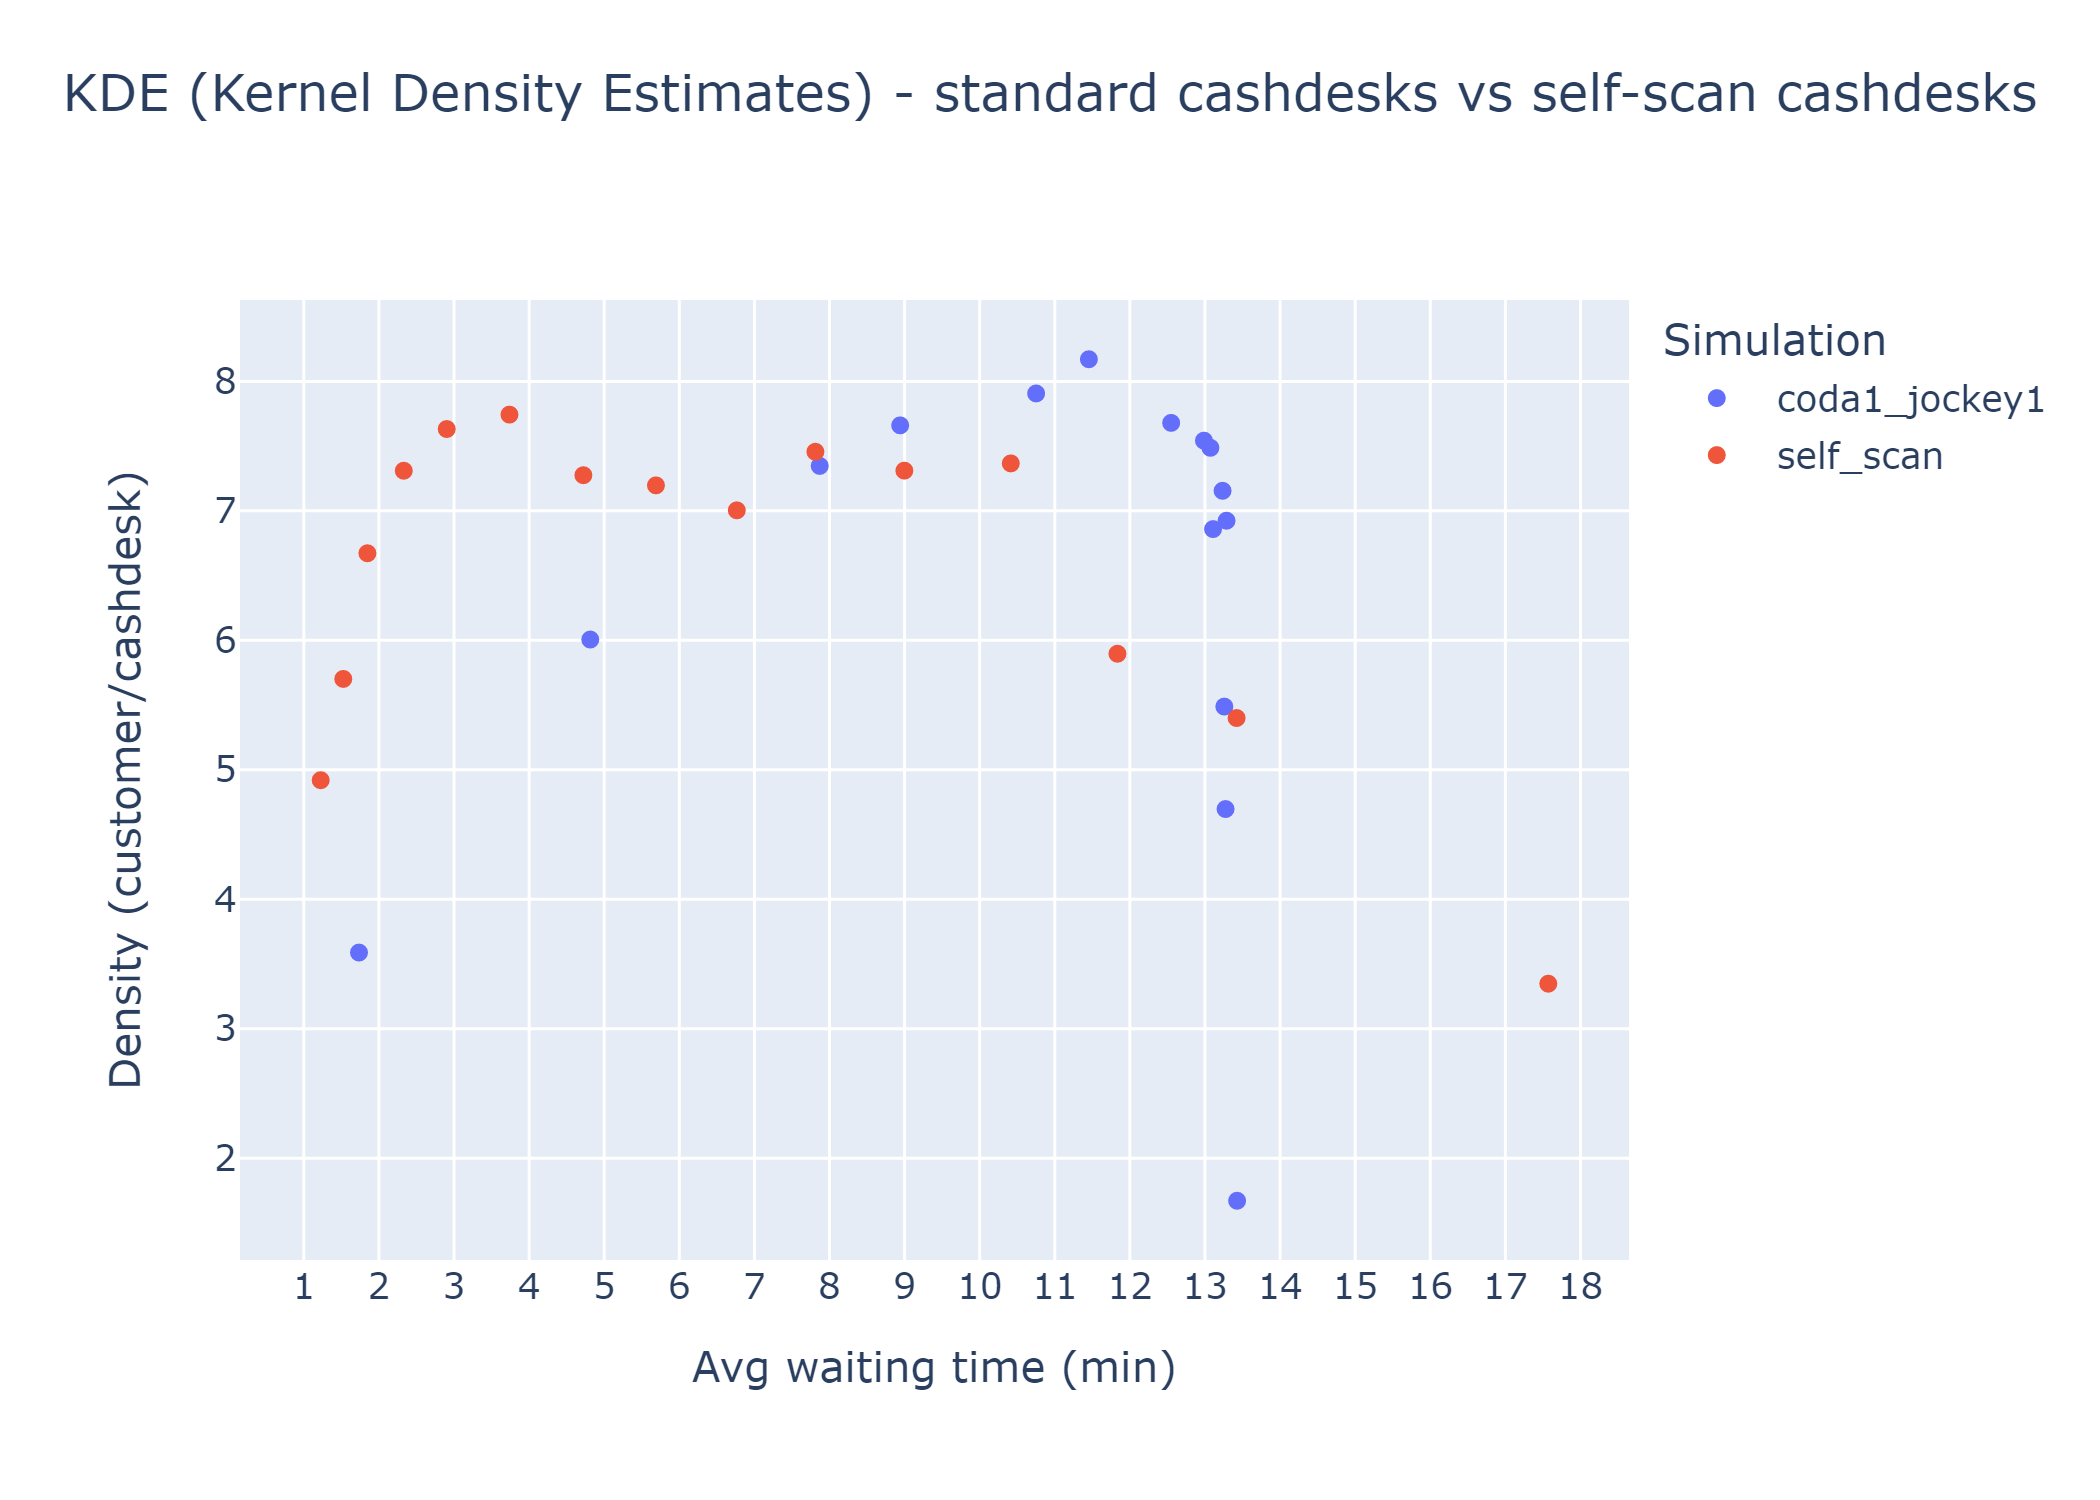
\includegraphics[width=8cm]{"../report/images/results/kde_self_scan.png"}
	\end{figure}
	Le casse standard gestiscono il momento di massima densità abbassando i tempi medi d'attesa, le self-scan no.
\end{frame}

\begin{frame}{Simulazione non deterministica}
	Introduciamo i parametri randomici per rendere la simulazione più verosimile, e non per abbassare i tempi d'attesa. I parametri sono:
	\begin{itemize}
		\item 20 casse standard
		\item 6 casse self-service
		\item 5 casse self-scan
		\item Probabilità cliente self-scan: $50 \%$
		\item Errore di stima della quantità di elementi nei carrelli con $0.1$ di deviazione standard
		\item 4 strategie di scelta della coda
		\item 2 strategie di jockey
	\end{itemize}
	Per un totale di 8 simulazioni.
\end{frame}

\begin{frame}{Simulazione non deterministica}
	\begin{figure}[H]
		\centering
		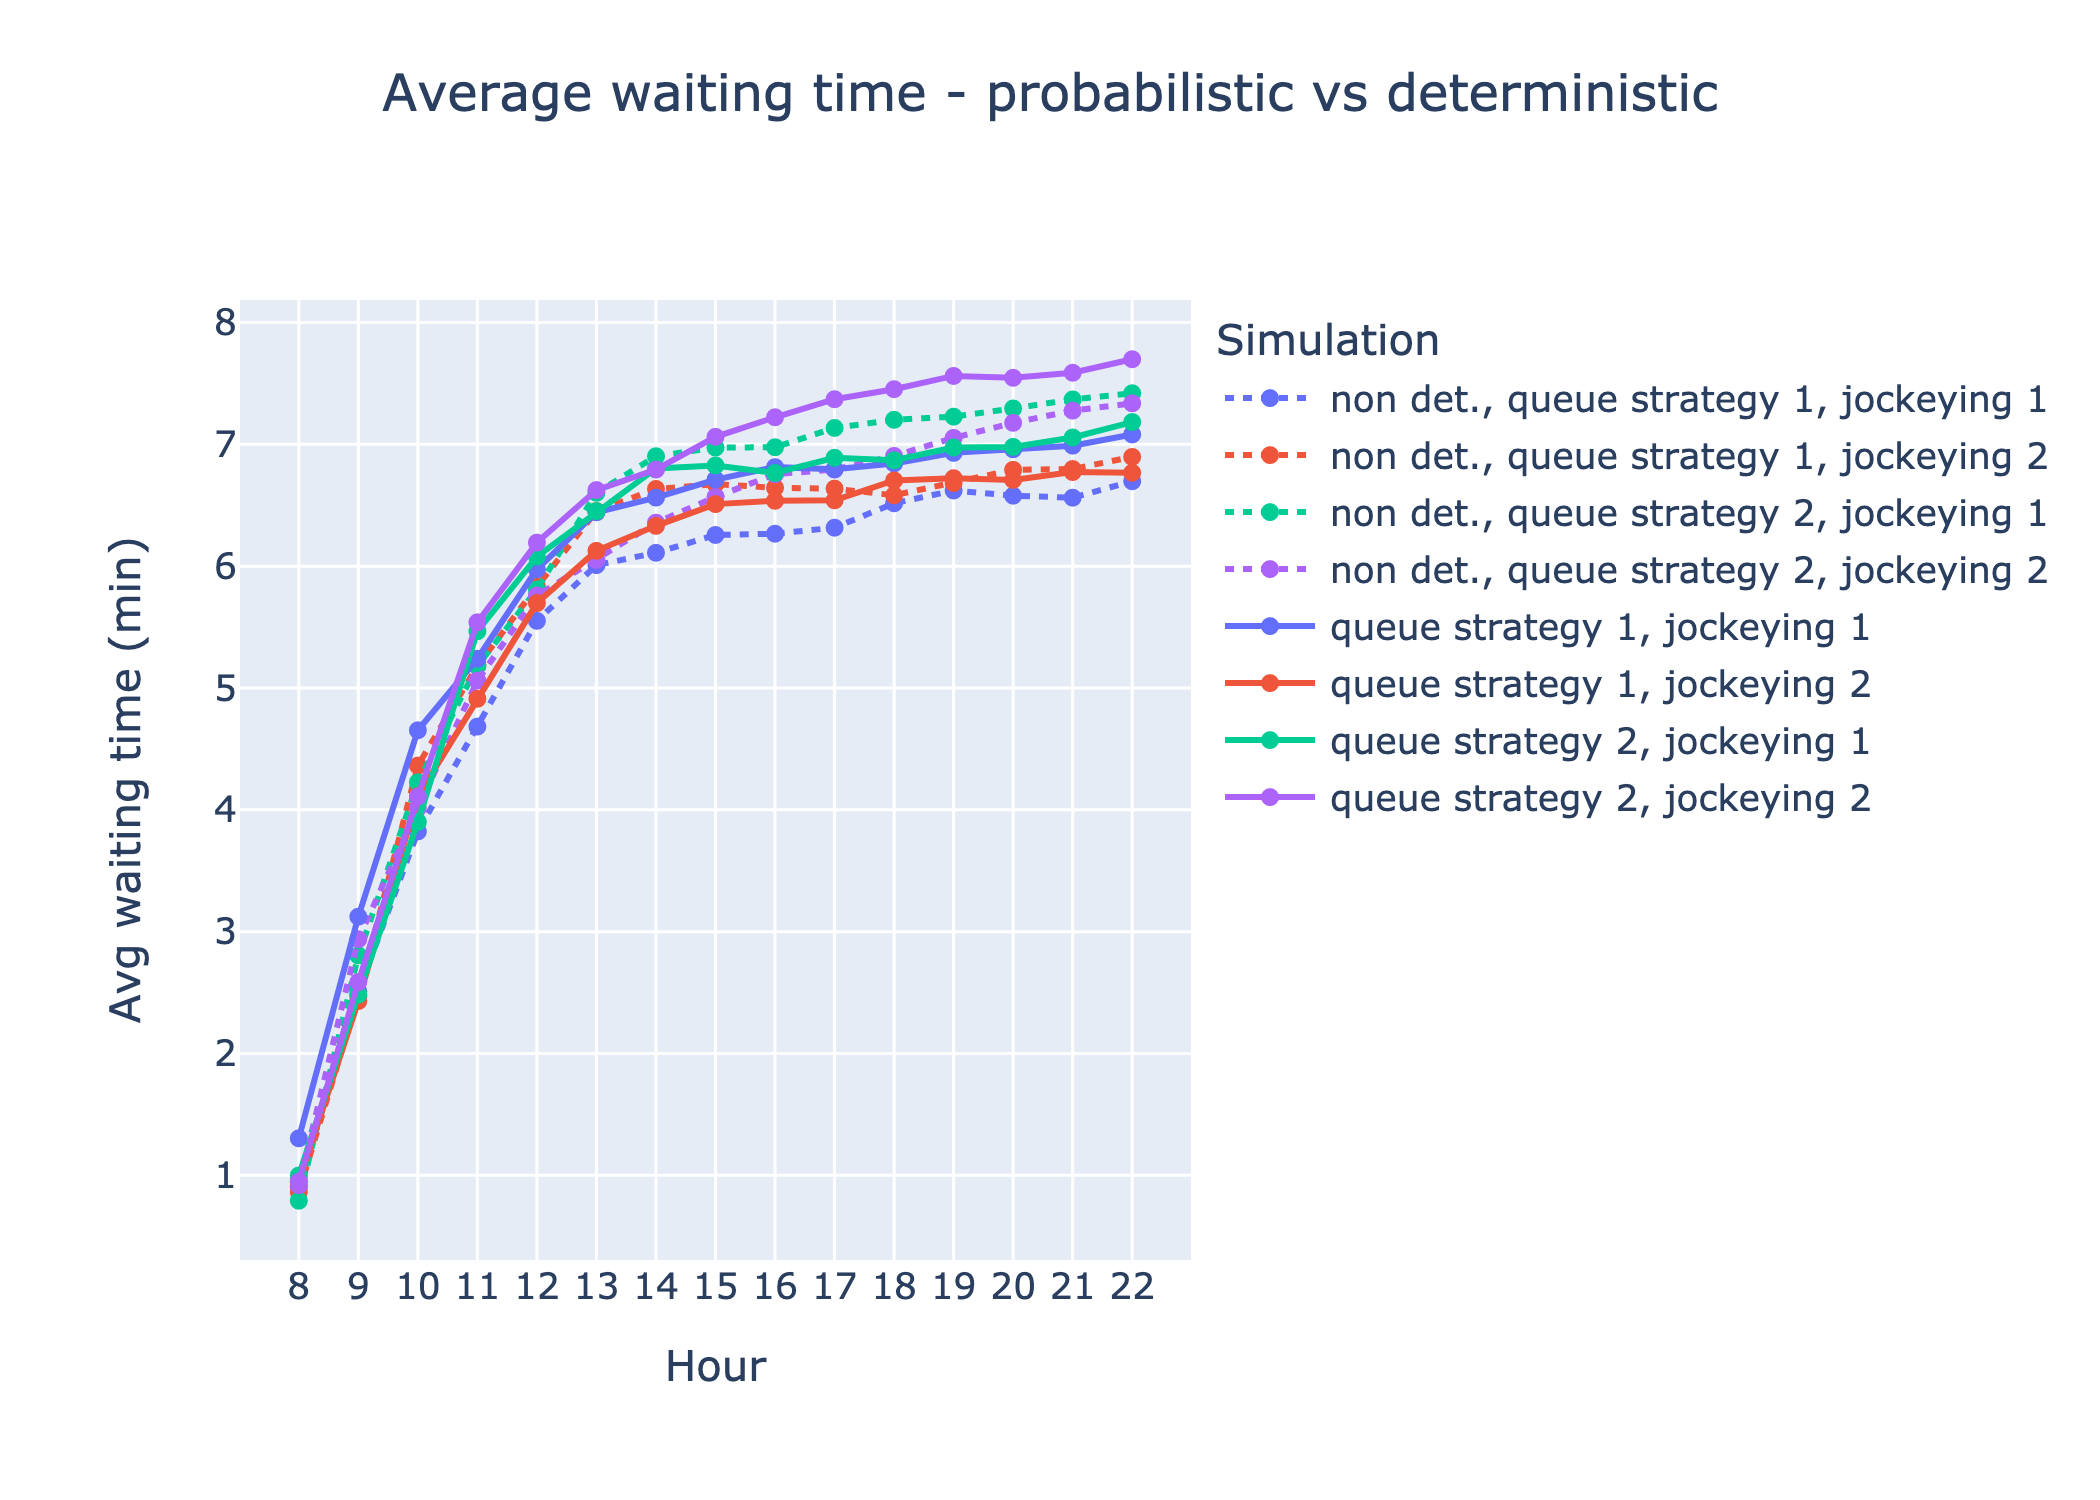
\includegraphics[width=8cm]{"../report/images/results/avg_wt_prob.png"}
	\end{figure}
	I tempi medi sono paragonabili per tutte le strategie, osserviamo quindi che i parametri randomici introdotti sono pensati con il buon senso e non scombinano il modello. Servono a simulare più scenari possibili.
\end{frame}